\section{Alex Pitcher Report - Ben Banfield}

\fullwidthbox[\award]{The Alex Pitcher Memorial Award}{
     The Alex Pitcher Memorial Award is an individual grant from the Ghar Parau Foundation (GPF) awarded to young cavers. Alex Pitcher was a young caver who lost his life on an expedition to the \passage{Gouffre Berger} in the late 1980s. His memorial fund was established to support young cavers (under the age of 25) going on their first expedition outside the UK or Ireland. It is usually put towards training and/or personal equipment costs for such individuals. One or two awards are made each year per GPF Expedition Grant Application, in the order of £100 each.}

This summer I was a member of Imperial College Caving Club's expedition
to \passage[mountain]{Tolminski Migovec} in the Julian Alps in Slovenia. The club has been
running the expedition for over a decade now and I was looking forward to
improving my caving skills and techniques as well as contributing to the
knowledge about the caves under the \passage{Migovec plateau}. The Alex Pitcher
Memorial Fund kindly awarded me some money which helped me purchase my
own helmet and helmet mounted light. Having my own helmet mounted light
was essential to my participation in the expedition, as the club only
owns FX3's with batteries on a belt that are unsuitable for \passage{Migovec} due
to the batteries needing a mains. Below is a report of most of my caving
activities during the expedition.

\subsection{Wednesday 18th (July)}

After being suggested as \bignote{a lead with a lot of potential and a good place
for budding cave explorers}, Tom Brown and myself set off for \passage{Moth Cave},
in shorts, t-shirts, knee-pads and helmets for a look. Spent a few hours
shifting boulders and scree 15 m into the cave at the pushing front,
before leaving. Has a gusting draught at the pushing front. Will return
again with tools and proper clothing for a better look.

\subsection{Thursday 19th}

\margininbox{Moth Cave}{
     \begin{itemize}
    \item Ben Banfield
    \item Tom Brown
    \item Alvin Chow
    \end{itemize}}{\explo}

Alvin joined Tom and myself today to continue pushing the lead in \passage{Moth
Cave}. After a few rotations of digging we had a badger sized hole and
decided to stop for lunch. Afterwards more excavating around the \passage{Badger
Hole} and scree slope occurred. Several animal bones were recovered from
the scree. An ominous slab of rock sat at the top of the scree making
progress tenuous. Further digging around the badger hole led to another
badger sized tunnel off to the left of the original. After moving 45-50
bags of scree we called it a day. Out 8pm with plans to ask about
explosives for further pushing.

\begin{figure*}[t!]
\checkoddpage \ifoddpage \forcerectofloat \else \forceversofloat \fi
\frame{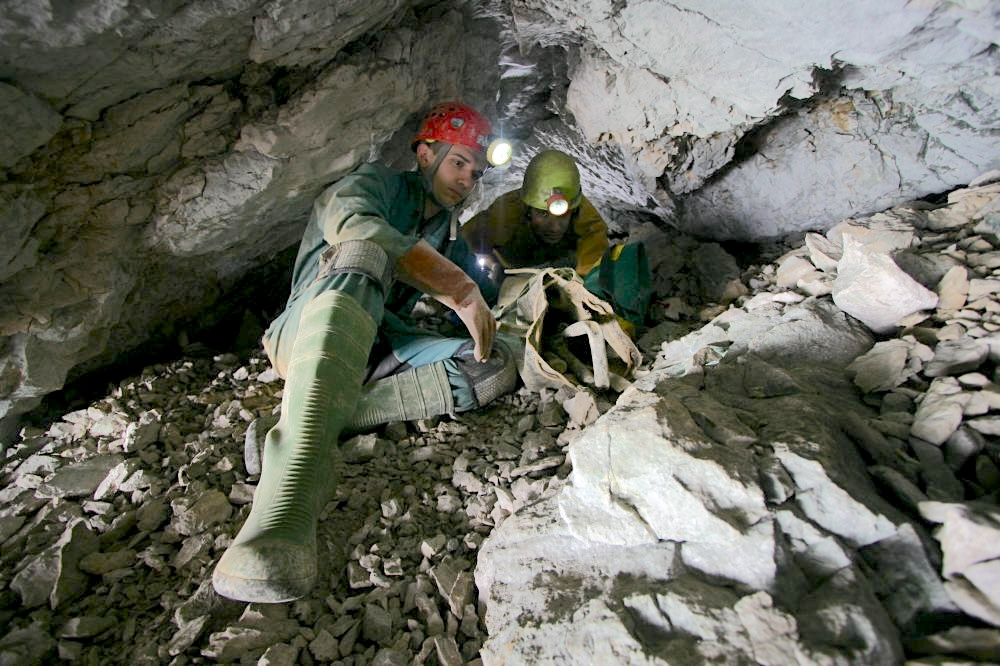
\includegraphics[width=\linewidth]{2007/ap_memorial_award/martin mcgowan -sandeep and ben in moth cave entrance--orig.jpg}}
\caption{Ben and Sandeep in the entrance to \protect\passage{Moth Cave}. \pic{Martin McGowan}}
\end{figure*}

\subsection{Friday 20th}

A short look at \passage{Moth Cave} with t-shirts and shorts again with Martin to ask
about explosives and other digging options. \bignote{Moved the ominous boulder at
the top of the scree to ease our minds} about becoming crushed. The
bottom of the scree slope was dug to more resemble a trench for easier
access to the pushing front.

\subsection{Sunday 22nd}

With the potential for leads and the fact that \passage{Moth Cave} lies on top of the
\passage{System Migovec} / \passage{Primadona} connection area, linking it into the
main survey was a priority. Martin taught several of us the essentials
of surveying while we surface surveyed to \passage{Moth Cave} entrance. Alvin and Thara
continued digging while Martin, Tom and myself surveyed to the pushing
front. 6 survey stations later we joined up with the digging team. Using
various combinations of left and right-handers we made a lot of progress
expanding the left hand badger hole and the trench. \bignote{Breakthrough looking
likely tomorrow}.

\subsection{Tuesday 24th}

After a day's break I rejoined the \passage{Moth Cave} pushing team. Sandeep had joined
us and almost straight away he managed to squeeze through the tunnel
(now named \passage{Badger Highway}) and into a small chamber. Alvin and myself
then made it through and throughout the afternoon work commenced on
enlarging \passage{Badger Highway} from the other end, to make it accessible to
larger cavers. The chamber contained going leads. One, a long
crawl/squeeze that needed enlarging had most potential.

\subsection{3rd week of expedition}

After proving to be such a promising lead before the expedition and
during the first two weeks, \passage{Moth Cave} needed the final push to see
whether it goes or dies. The day prior the petrol drill joined us to try
and enlarge \passage{Badger Highway} to allow more people to reach the pushing
front. Unfortunately the drill was more of a hindrance than a help,
fuming the cave and not expanding the passage.

\begin{marginfigure}
\frame{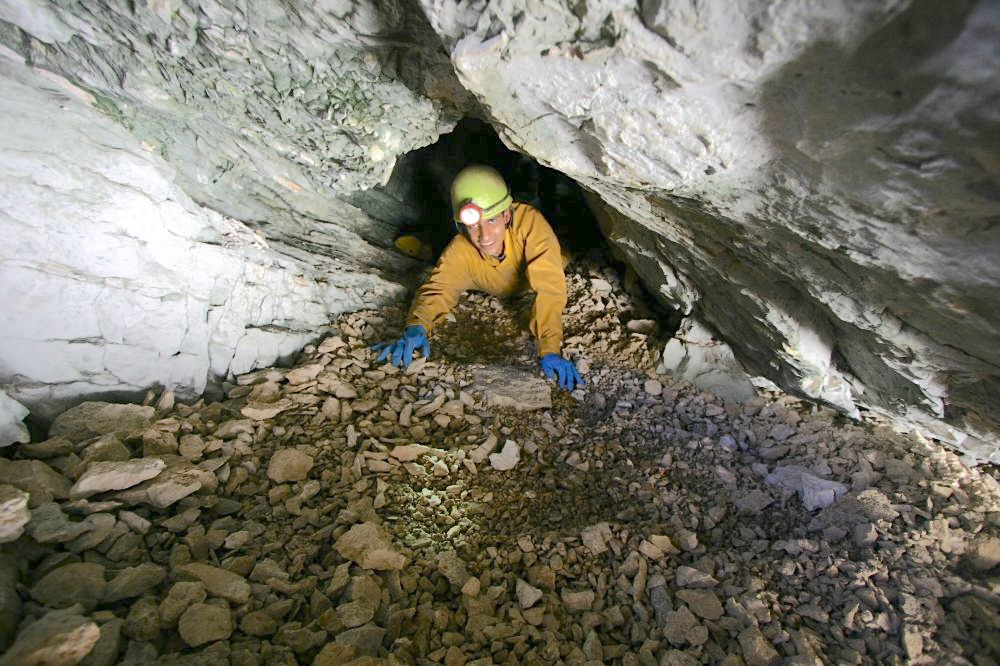
\includegraphics[width=\linewidth]{2007/ap_memorial_award/martin mcgowan -sandeep in moth cave--orig.jpg}}
\caption{Sandeep in the entrance to \protect\passage{Moth Cave}. \pic{Martin McGowan}}
\end{marginfigure}

With no draught coming from the pushing front or even through \passage{Badger
Highway} any more, hopes for a breakthrough didn't look promising.
Everyone else had plans for the next day, so armed with a survey kit and
some bright red nail varnish, I took on the mission of completing the
survey and exploring all available leads.

The squeeze through the tunnel looked more daunting than ever, but with
the knowledge a call-out team would be along within a few hours, I
pushed through. Minor digging allowed me further access along the main
lead. Another small chamber with no going leads was found. The nail
varnish came in useful to mark a permanent survey station. Taking all
digging tools and the survey notes out, I was back to camp well before
my call-out and in time for a nice rest in the sun.



\begin{pagefigure}
      \checkoddpage \ifoddpage \forcerectofloat \else \forceversofloat \fi
    \centering
    \begin{subfigure}{0.49\textwidth}
        \frame{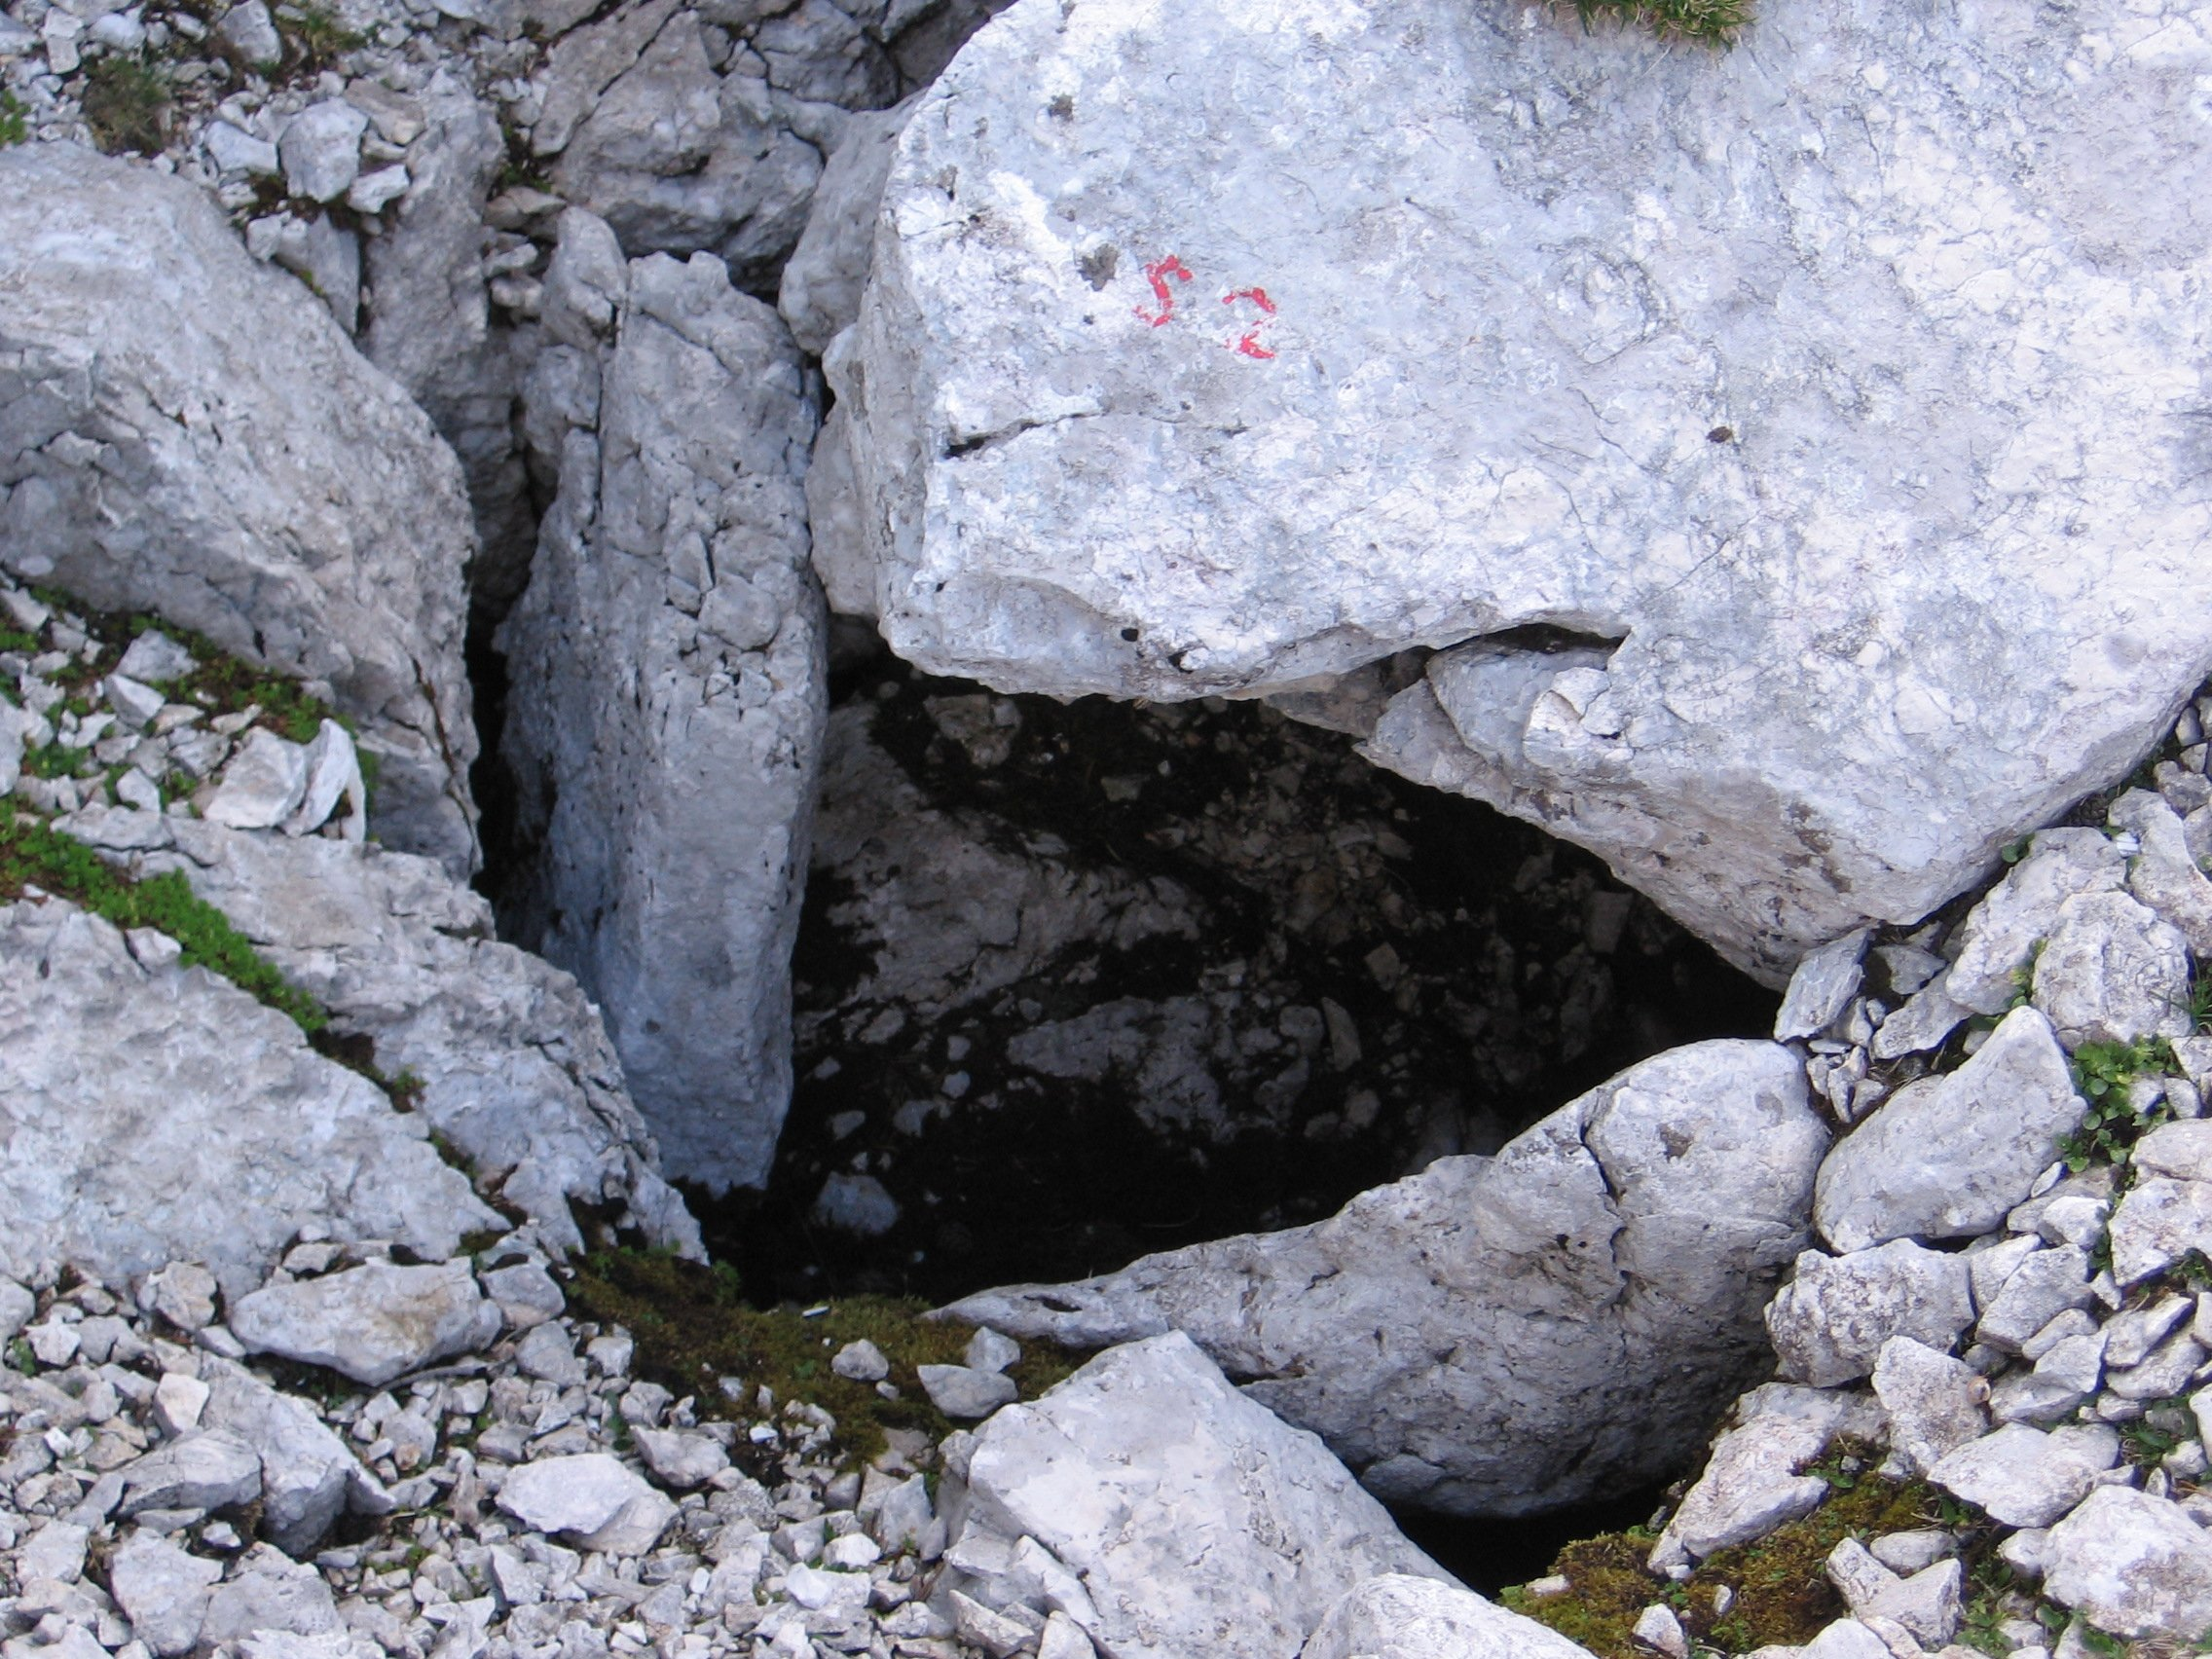
\includegraphics[width=\linewidth]{2007/S/jarvist frost - s2 entrance--orig.jpg}}
        \caption{\protect\passage{S2}}
    \end{subfigure}
\hfill
    \begin{subfigure}{0.49\textwidth}
    \centering
        \frame{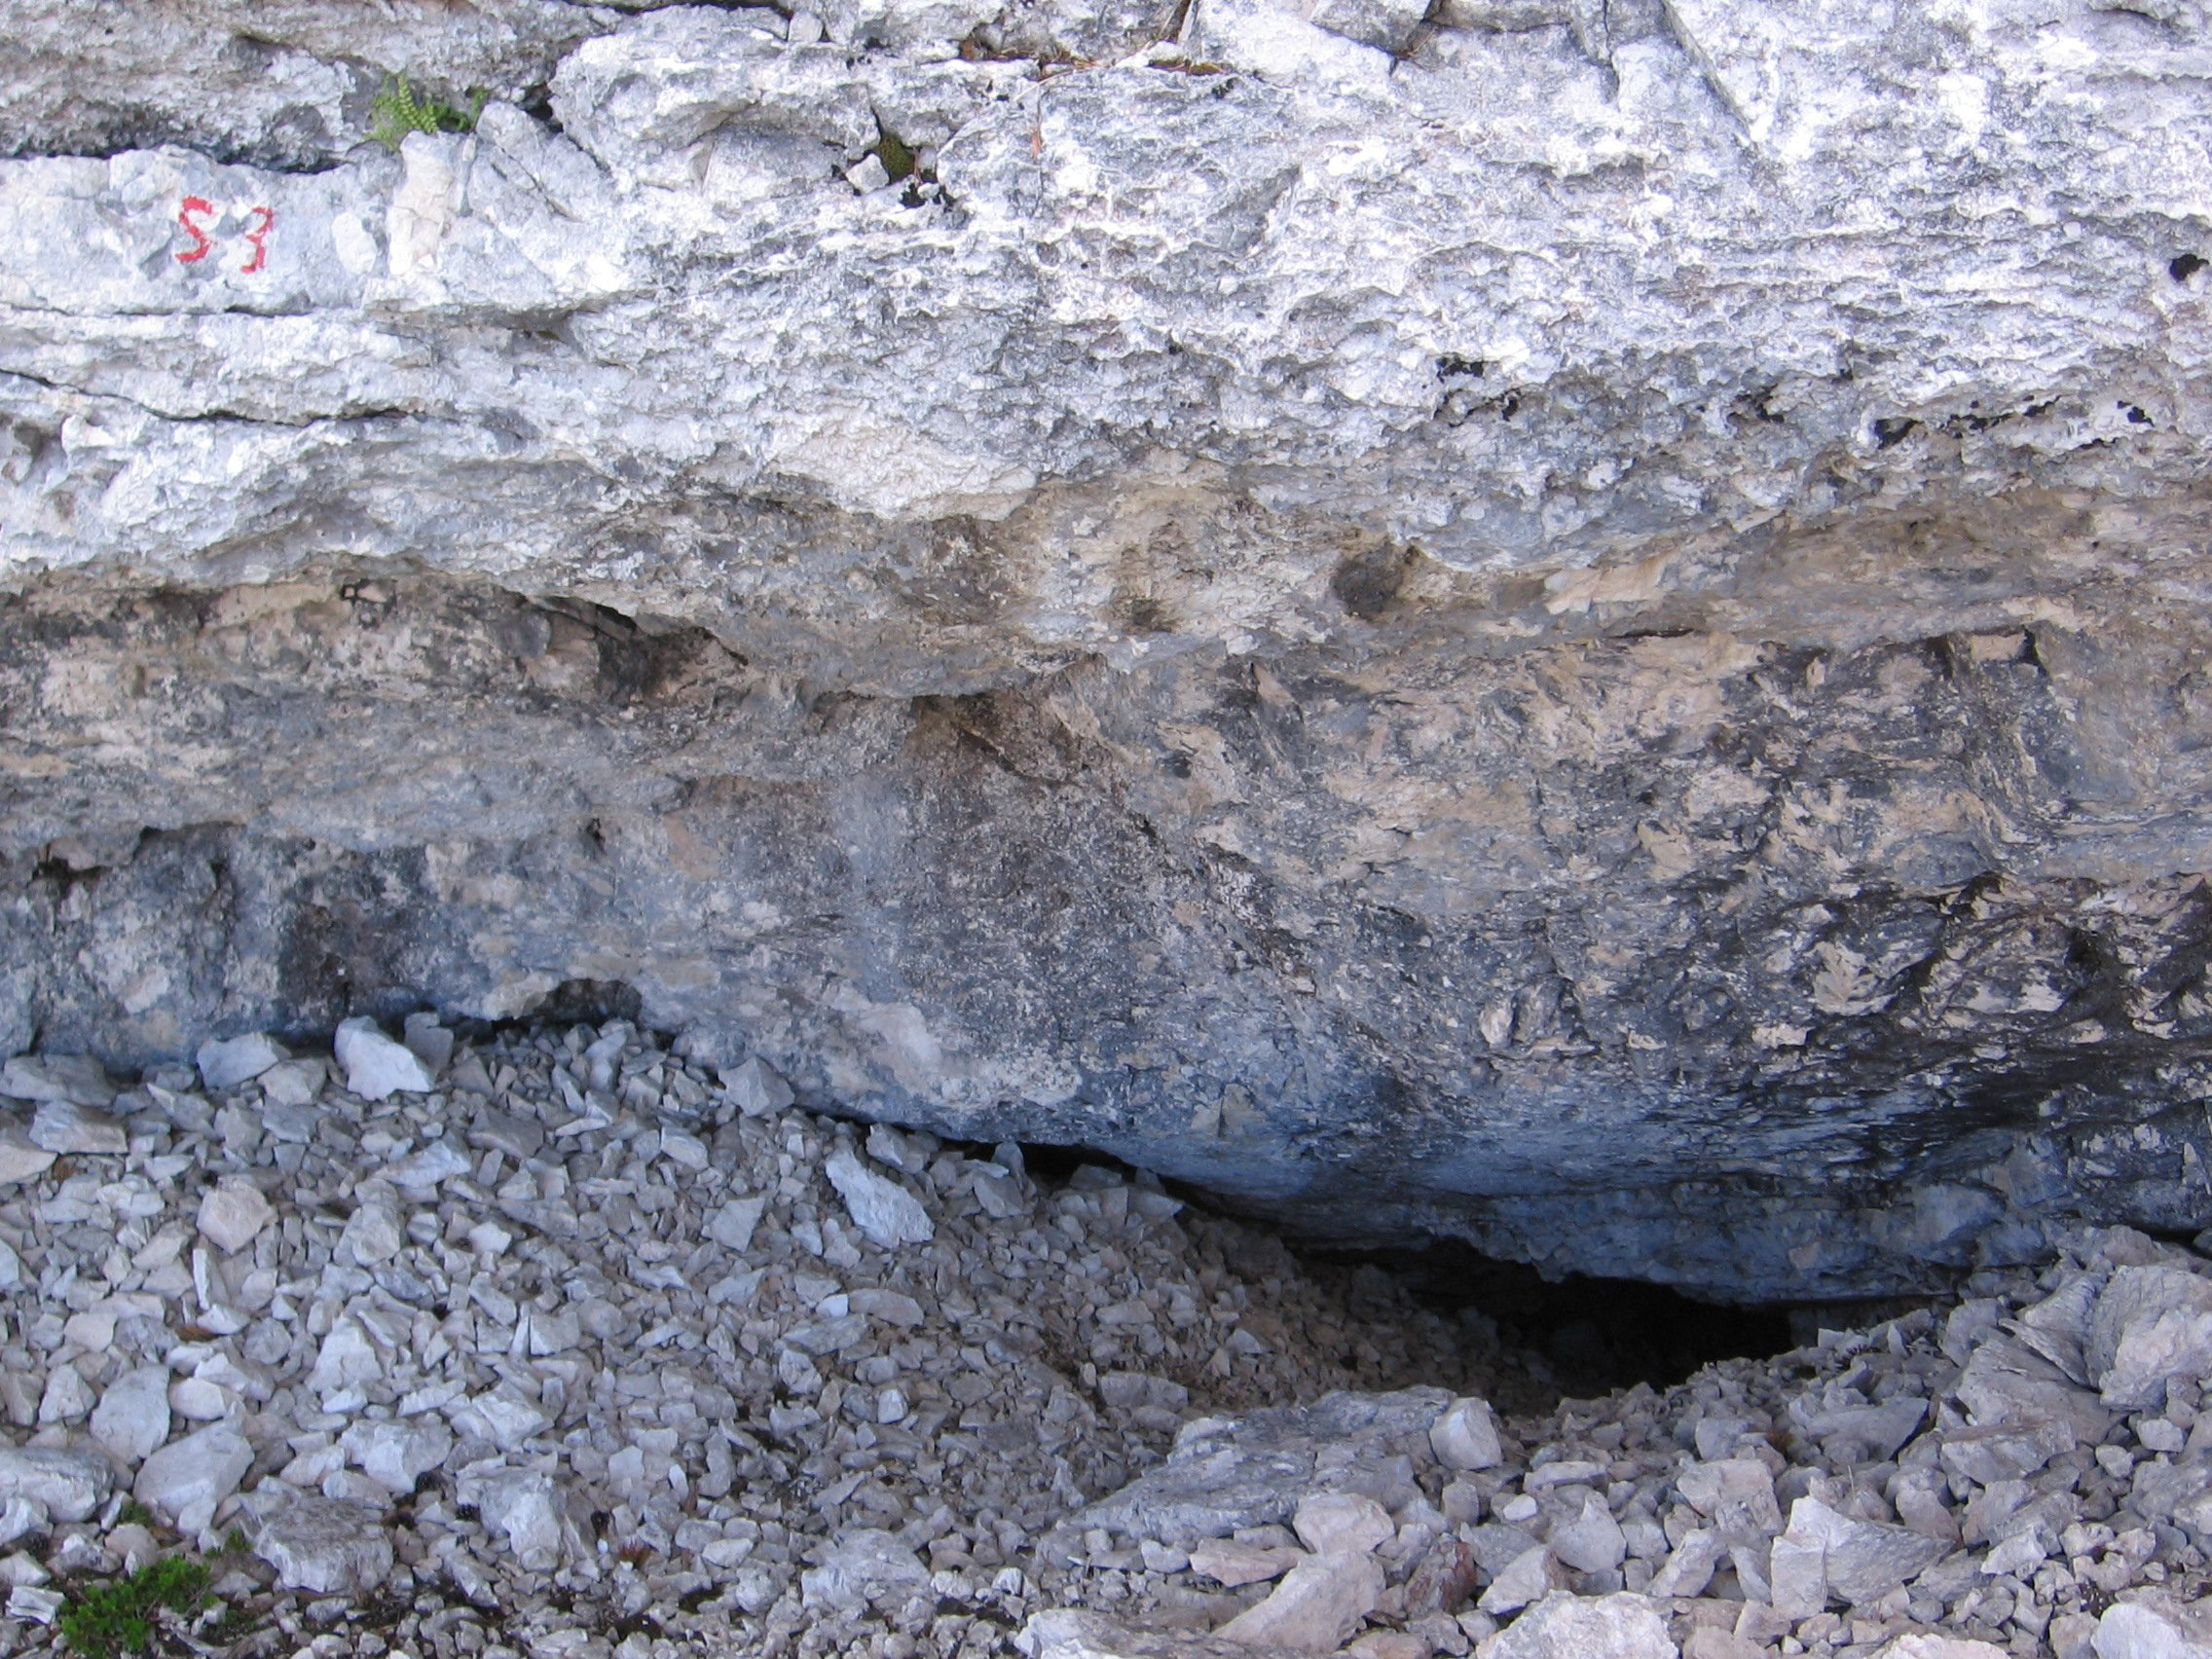
\includegraphics[width=\linewidth]{2007/S/jarvist frost - s3 entrance--orig.jpg}}
        \caption{\protect\passage{S3}}
\end{subfigure}
\vfill
\begin{subfigure}{0.49\textwidth}
    \centering
        \frame{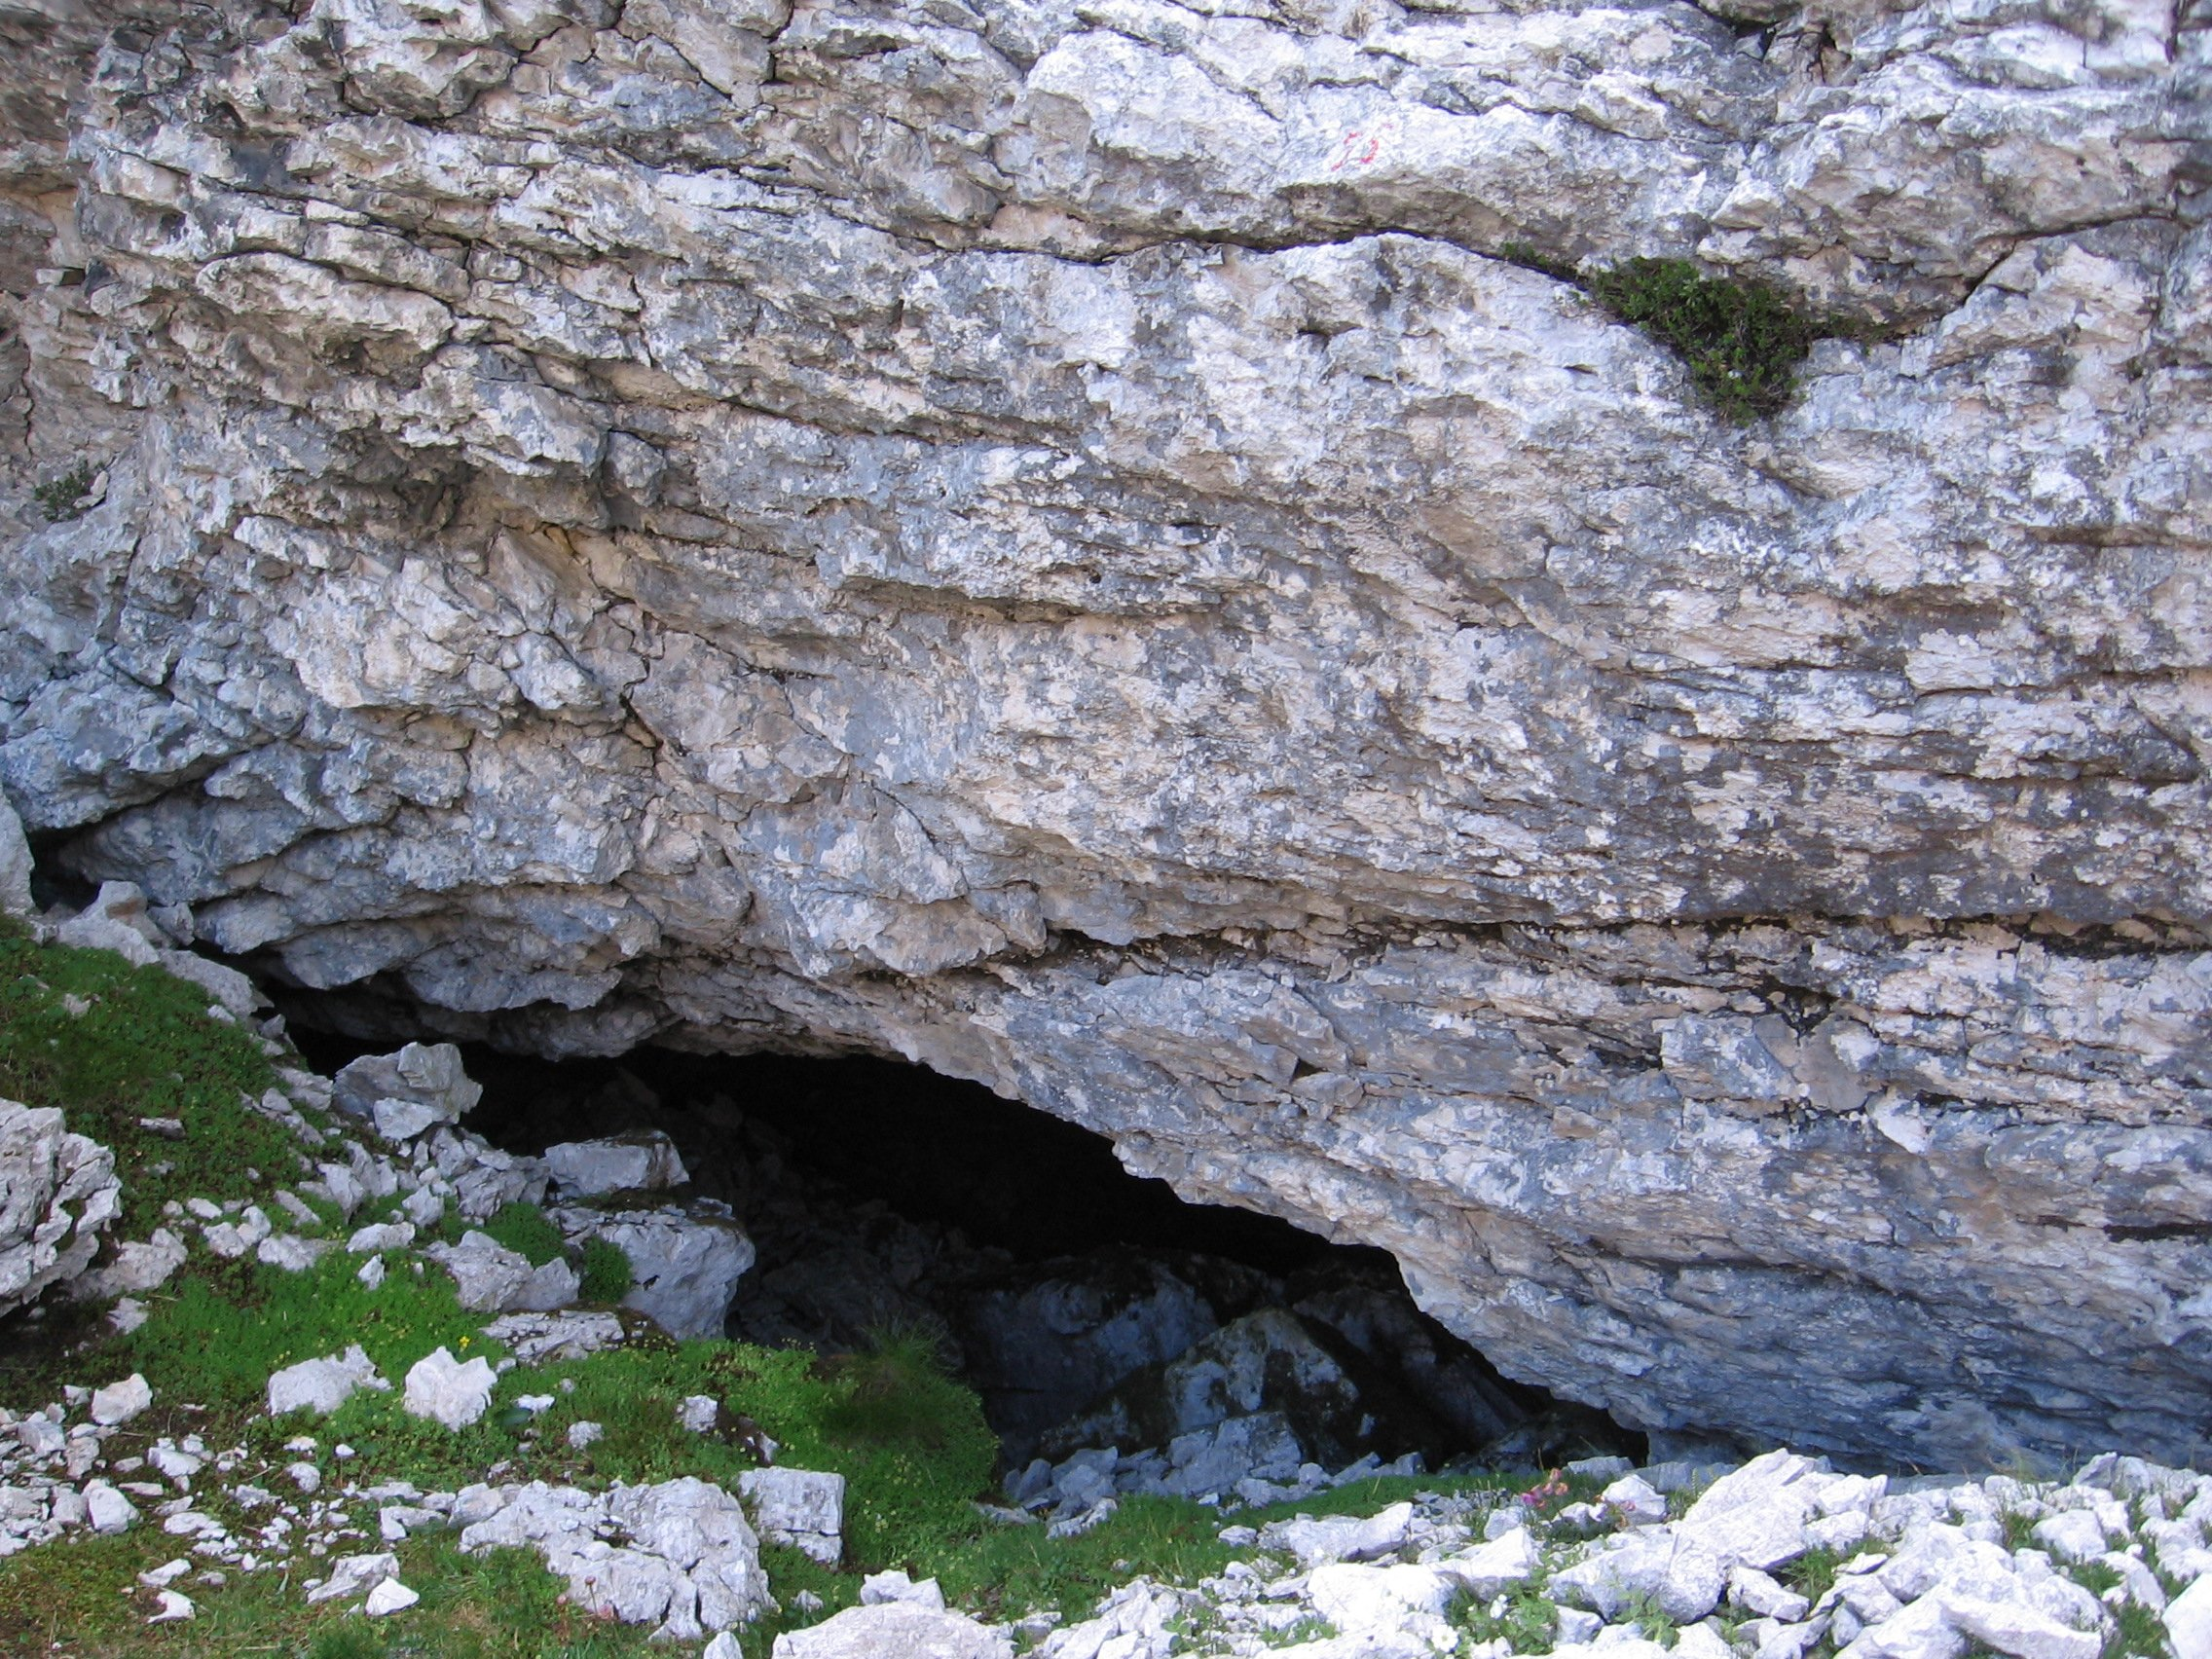
\includegraphics[width=\linewidth]{2007/S/jarvist frost - s5 entrance--orig.jpg}}
        \caption{\protect\passage{S5}}
\end{subfigure}
\hfill
\begin{subfigure}{0.49\textwidth}
    \centering
        \frame{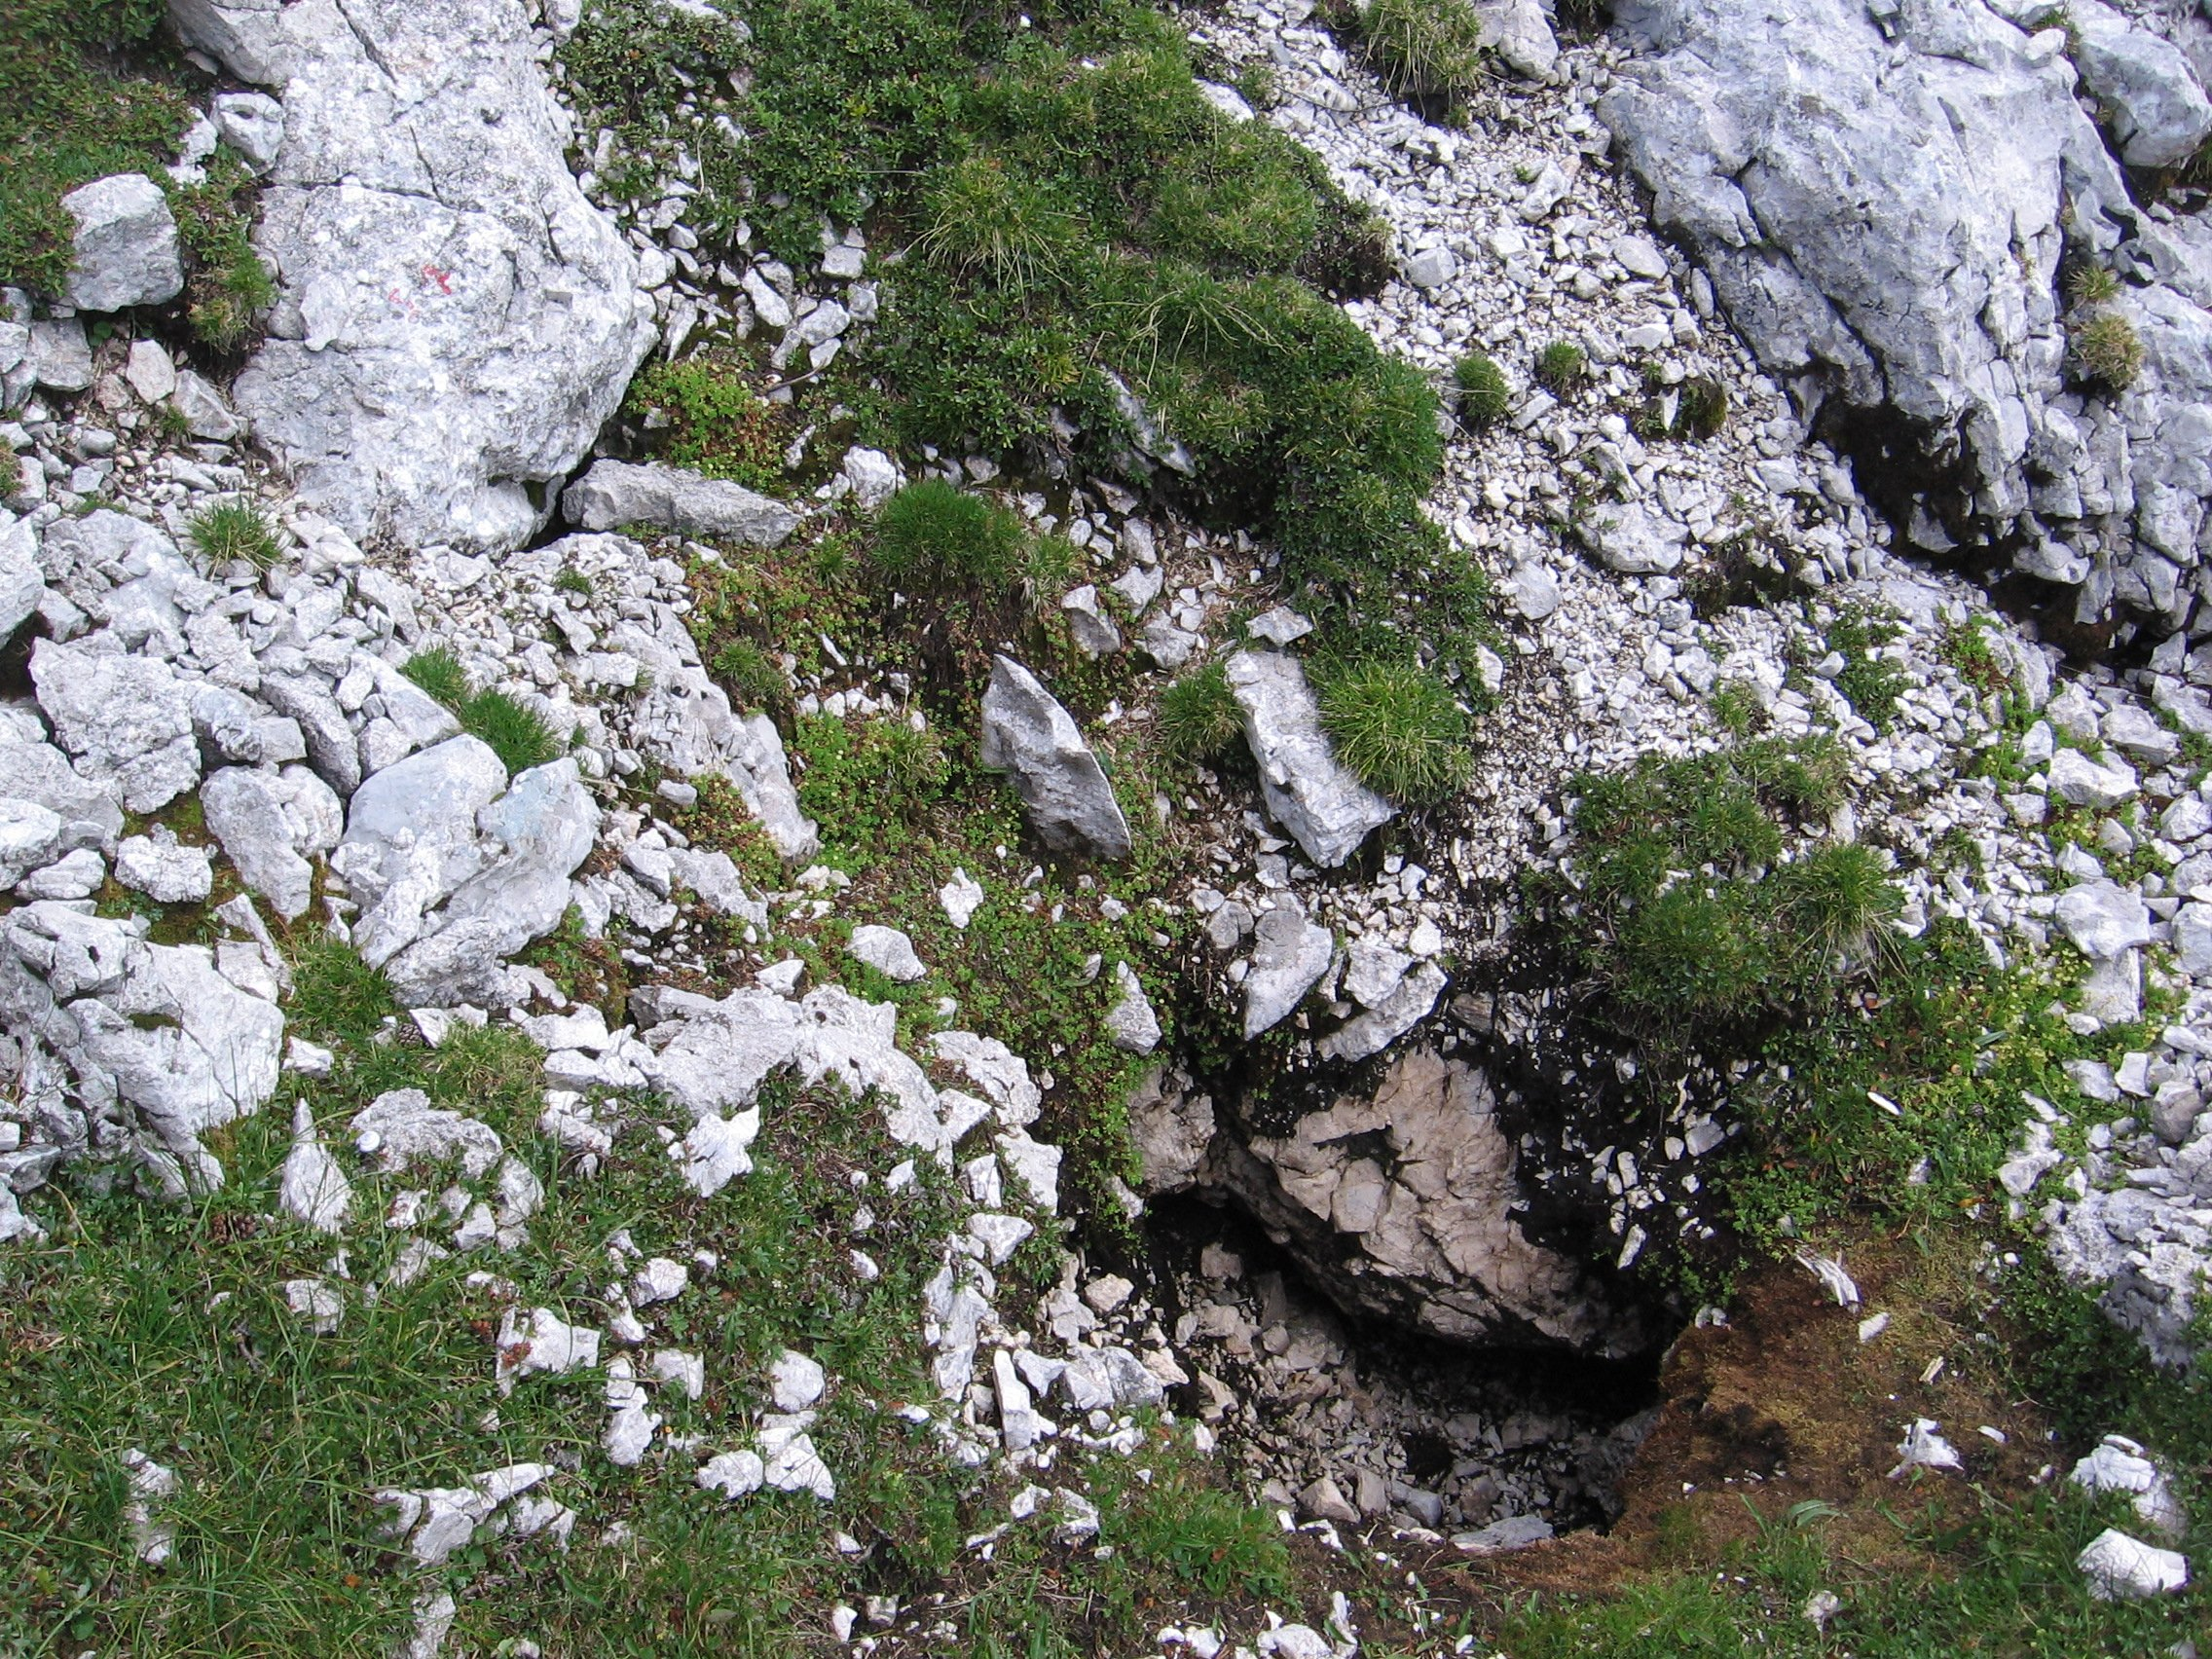
\includegraphics[width=\linewidth]{2007/S/jarvist frost - s7 entrance--orig.jpg}}
        \caption{\protect\passage{S7}}
    \end{subfigure}
\caption{Some of the entrances of the lesser-known holes in the S-series. \pic{Jarvist Frost}}
\end{pagefigure}



After a jolly into \passage{System Migovec} earlier in the week in a large group,
it was definitely time for me to go deep in a pair. What better way than
to help Rik push \passage{Captain Kangaroo}! With leads that had been looked at
but not surveyed, interesting data collection in scrott was the order of
the day. Down, down, down through the early \passage{Gardeners' World} pitches and
past some ``interesting'' rigging (greatly improved later in the
expedition). Squiggling through the rifts in \passage{Scrotty} until we reached
\passage{Traverse Chamber}. The first lead ended quickly in a pitch preceded by a
tight squeeze past a spiney. With no rope and no hammer to help make the
entrance more accessible let alone rigging, it was impossible for now.
After surveying back to a fork, we pushed on.

What followed was a crash course in free climbing as taught by Rik.
Plenty of top tips later, we made it past the fiddly squeeze where Rik
and Jarvist turned back at the last exploration. Beyond was an open
chamber. Rik climbed down and \bignote{suddenly \passage{Captain Kangaroo} became a whole
lot more exciting}. A pitch, two going rifts and horizontal walking
passage. The climb was do-able, but really needed rigging, so we turned
and surveyed back to \passage{Traverse Chamber}. Out an hour early, we hurried
back to camp for slop. As our survey data, excitement mounted. Our data
was heading towards \passage{System Migovec} for the mythical connection. The
laptop was whipped out and data entered. Our survey came within 36 m of
the bottom \passage{M2} below \passage{Silos}! A bit of rope and some further pushing
and we'll be there. Roll on the survey legs!

I found the expedition an extremely enjoyable and fulfilling experience.
I gained a lot of valuable caving experience. The exploration and
discovery of new cave passage was very rewarding. Having my waist freed
from wearing a battery belt, made caving in tight passageway and
squeezes immeasurably easier. I would like to thank the Ghar Parau
Foundation and the Alex Pitcher Memorial Fund for helping me on my first
caving expedition.

\name{Ben Banfield}

